\documentclass[a4paper,
			   11pt,
			   ngerman, 
			   ]{scrreprt}

\usepackage[left=2.5cm,right=2.5cm,top=2.5cm,bottom=2.5cm]{geometry}
\usepackage{lipsum}
\usepackage[utf8]{inputenc}
\usepackage{csquotes}
\usepackage{graphicx}
\usepackage[section]{placeins}
\usepackage{fontenc}
\usepackage[automark]{scrlayer-scrpage}
\usepackage[ngerman]{babel}
\usepackage[natbib=true,style=numeric, sorting=none]{biblatex}



%%%%%%%%% KOPFZEILE %%%%%%%%%%%%%%%%%%%%%
\pagestyle{scrheadings} 
\chead*{\headmark}
\cfoot*{\pagemark}

\addbibresource{ref/ref.bib}

\publishers{
	\begin{tabular}{rl} %jedes C für eine spalte c für centered

		Erstprüfer: & Prof. Dr. Christian Pfitzner \\
		Betreuer:   & Prof. Dr. Christian Pfitzner \\
		Ausgabedatum: & 23.03.2023 \\
		Abgabedatum: & 20.06.2023 \\
	\end{tabular}
}


\begin{document}

	%%%%%%%%% KOPF %%%%%%%%%%%%%%%%%%%%%%%%%%
	\title{Seminararbeit}
	\subtitle{Sensorik-gestützte Robotik-Systeme zur Automatisierung landwirtschaftlicher Prozesse}
	\author{Nico Elsner\\
	Studiengang: Robotik}
	\date{\today}
	\maketitle
	\tableofcontents
	\thispagestyle{empty}
	%%%%%%%%%% EINLEITUNG %%%%%%%%%%%%%%%%%%%
	\newpage
	\setcounter{page}{1}
	\chapter{Einleitung}
	In den vergangenen Jahrzehnten entwickelte sich durch das steigende
Bevölkerungswachstum ein weltweiter Mangel an Ressourcen, vor allem an
Nahrungsmitteln.\\Die Folge
hiervon sind Massentierhaltung, Monokulturen und Gewächshausplantagen. Der
Trend geht zur Perfektion der Erträge, bei möglichst geringem Aufwand. Dabei
wird der Fokus darauf gelegt, die vorhandene Fläche optimal zu nutzen, um viele
Lebensmittel auf geringem Raum zu produzieren. Dabei wird außerdem darauf
geachtet, den Ertrag der vorhandenen Pflanzen zu maximieren. Dies kann durch
eine intelligente Bewässerung, die Optimierung der Temperaturbedingungen, sowie
eine effiziente Bekämpfung von Unkraut und Schädlingen realisiert werden. Dabei
spielen Sensoren, zur Überwachung der Felder eine große Rolle. Aus den
Sensordaten können Robotersysteme erkennen, an welcher Stelle eine Aktion zur
Verbesserung Pflanzenbedingungen und damit der Maximierung des Ertrags
erforderlich ist. Ähnlich verhält es sich auch bei der Tierzucht, wobei Roboter
hierbei auch zum Wohl der Tiere durch Futterverpflegung und Stallreinigung
beigetragen wird. \\Auch in anderen Bereichen ist die Frage nach schnellen,
zuverlässigen Massenproduktionen bereits seit mehreren Jahrzehnten diskutiert.
\\Vorallem die Automobilindustrie hat bereits früh begonnen sich mit
Automatisierung zu beschäftigen. Erste Ansätze gab es hier bereits 1913 durch
Henry Ford, welcher die ersten Autos auf dem Fließband zusammenbauen ließ.
Dieses System wurde über die Jahrzehnte soweit ausgebaut, dass heutzutage
bereits viele Industrieroboter die Bandarbeit nahezu komplett autonom
erledigen. \\Jedoch gibt es auch in der Landwirtschaft bereits Ansätze, um die
Arbeit zu industrialisieren. \\In der folgenden Arbeit werden die fundamentalen
Grundlagen für eine effiziente Nutzung von sensorbasierten Robotersystemen
erläutert. Dabei wird auf bereits existierende Systeme aufgezeigt, die
benötigte Sensorik erläutert, sowie auf gesellschaftliche und technische
Herausforderungen eingegangen.
	\chapter{Hauptteil}
	
	In der Landwirtschaft gibt es viele Prozesse, die immer gleich sind. Solche Aufgaben sind perfekt dafür geeignet, um mithilfe von Robotik automatisiert zu werden. Zudem hat man bei Feldern, Äckern, etc. immer feste Ortspunkte und kann somit sehr gut mit GPS Koordinaten arbeiten.\\
	Im Folgenden wird auf die Grundlagen der benötigten Sensoren, sowie deren Flächenabdeckungsmöglichkeiten eingegangen.\\                                         Zudem werde ich einige bereits existierende Lösungsmöglichkeiten vorstellen und einen Ausblick geben, wie diese auf Industriegröße skaliert werden können.
	

	
	%%%%%%%%%%% ÜBERGREIFENDE SYSTEME %%%%%%%
	\chapter{Systeme}
		\section{Drohnen}
		In der Landwirtschaft geht es häufig darum, Sachen (Flüssigkeiten,Samen,etc.)
auf dem Feld auszubringen. Auf die herkömmliche Art macht das ein Bauer,
mithilfe eines Traktors. Je nach Aufgabe und Feldgröße benötigt ein Landwirt
hierfür mehrere kostbare Stunden. Die Ausbringung von Flüssigkeiten wäre ein
typischer Anwendungsfall für eine Drohne.

\begin{figure}[ht]
	\centering
	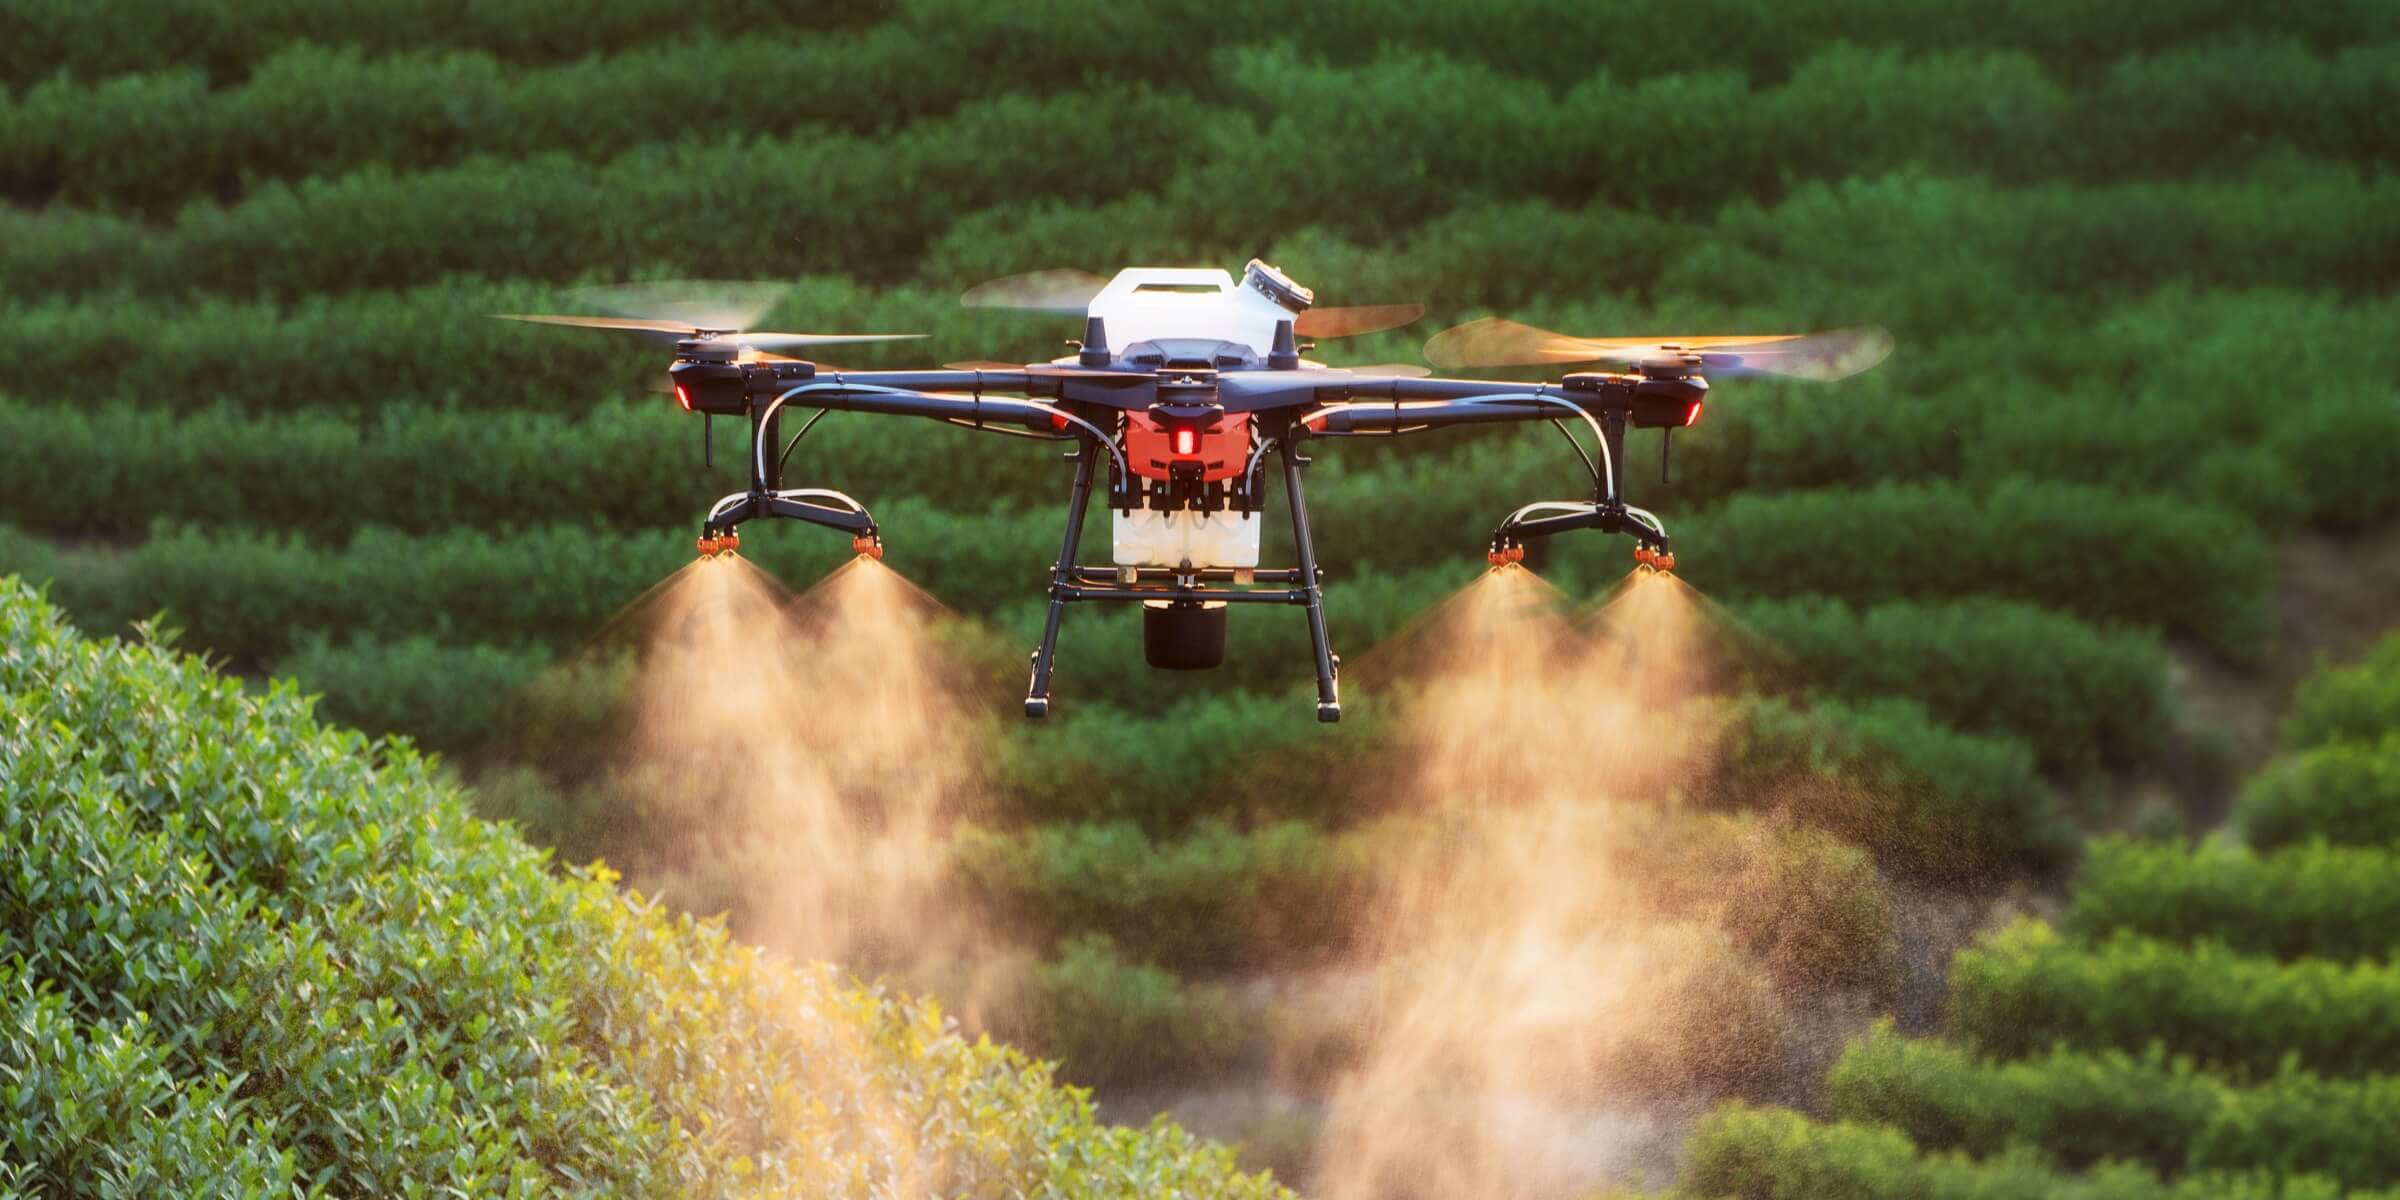
\includegraphics[width=0.7\textwidth]{bilder/drtohne.jpg}
	\caption[Sprühdrohne]{Sprühdrohne beim Aufbringen von Pestiziden \cite{Drohne}}
	\label{fig:sprühdrohne}
\end{figure}

Die Drohne in Abbildung \ref{fig:sprühdrohne} kann hierbei aus geringer Höhe
die entsprechenden Flüssigkeiten über eine Düse ausbringen. Das kann durch
Routenplanung komplett automatisiert passieren. Lediglich ein Flüssigkeitstank
ist hier benötigt, welcher jedoch innerhalb weniger Minuten vom Landwirt an
einer fest vorgegebenen Stelle platziert werden kann. Somit hat die Drohne
einen festen Bezugspunkt für das Auffüllen der Flüssigkeit, ähnlich einer
Ladestation eines Rasenmähers. \\ Ein zusätzliches weit verbreitetes
Einsatzgebiet von Drohnen im Allgemeinen ist die Überwachung: \\Auf den Feldern
wird dies häufig in Kombination mit Wärmebildkameras dazu verwendet, Tiere in
den Feldern aufzuspüren. Durch die Möglichkeit,
das Feld aus großen Höhen zu beobachten ermöglicht es dem Farmer, Rehe,
Wildschweine und andere Schädlinge schnell und effektiv in seinem Feld
aufzuspüren.

		\section{Schienensysteme}
		Unter Landwirtschaft zählen jedoch nicht nur klassische wie Äcker, Maisfelder, Getreidefelder, sondern unter anderem auch Gewächshäuser.
Auch in Gewächshäusern gibt es viele Aufgaben, welche durch Sensoren ersetzt, bzw. sogar verbessert werden können.
Der große Vorteil in Gewächshäusern ist die statische Umgebung.
Gemeint ist hiermit die festen Punkte, an welchen die Pflanzen wachsen. 
Dies ermöglicht dem Robotersystem eine ähnliche Arbeitsumgebung wie in einem Warenhaus in welchem die Systeme bestimmte Positionen und Höhen anzufahren.
Durch diese festen Bewegungspunkte ergibt sich die Möglichkeit eines Schienensystems, welches bereits in den vorher erwähnten Warenhäusern seinen Einsatz findet.
Hier gibt es bereits ein bekanntes Beispiel aus der Heimbeet-Szene:\\

\begin{figure}[ht]
	\centering
	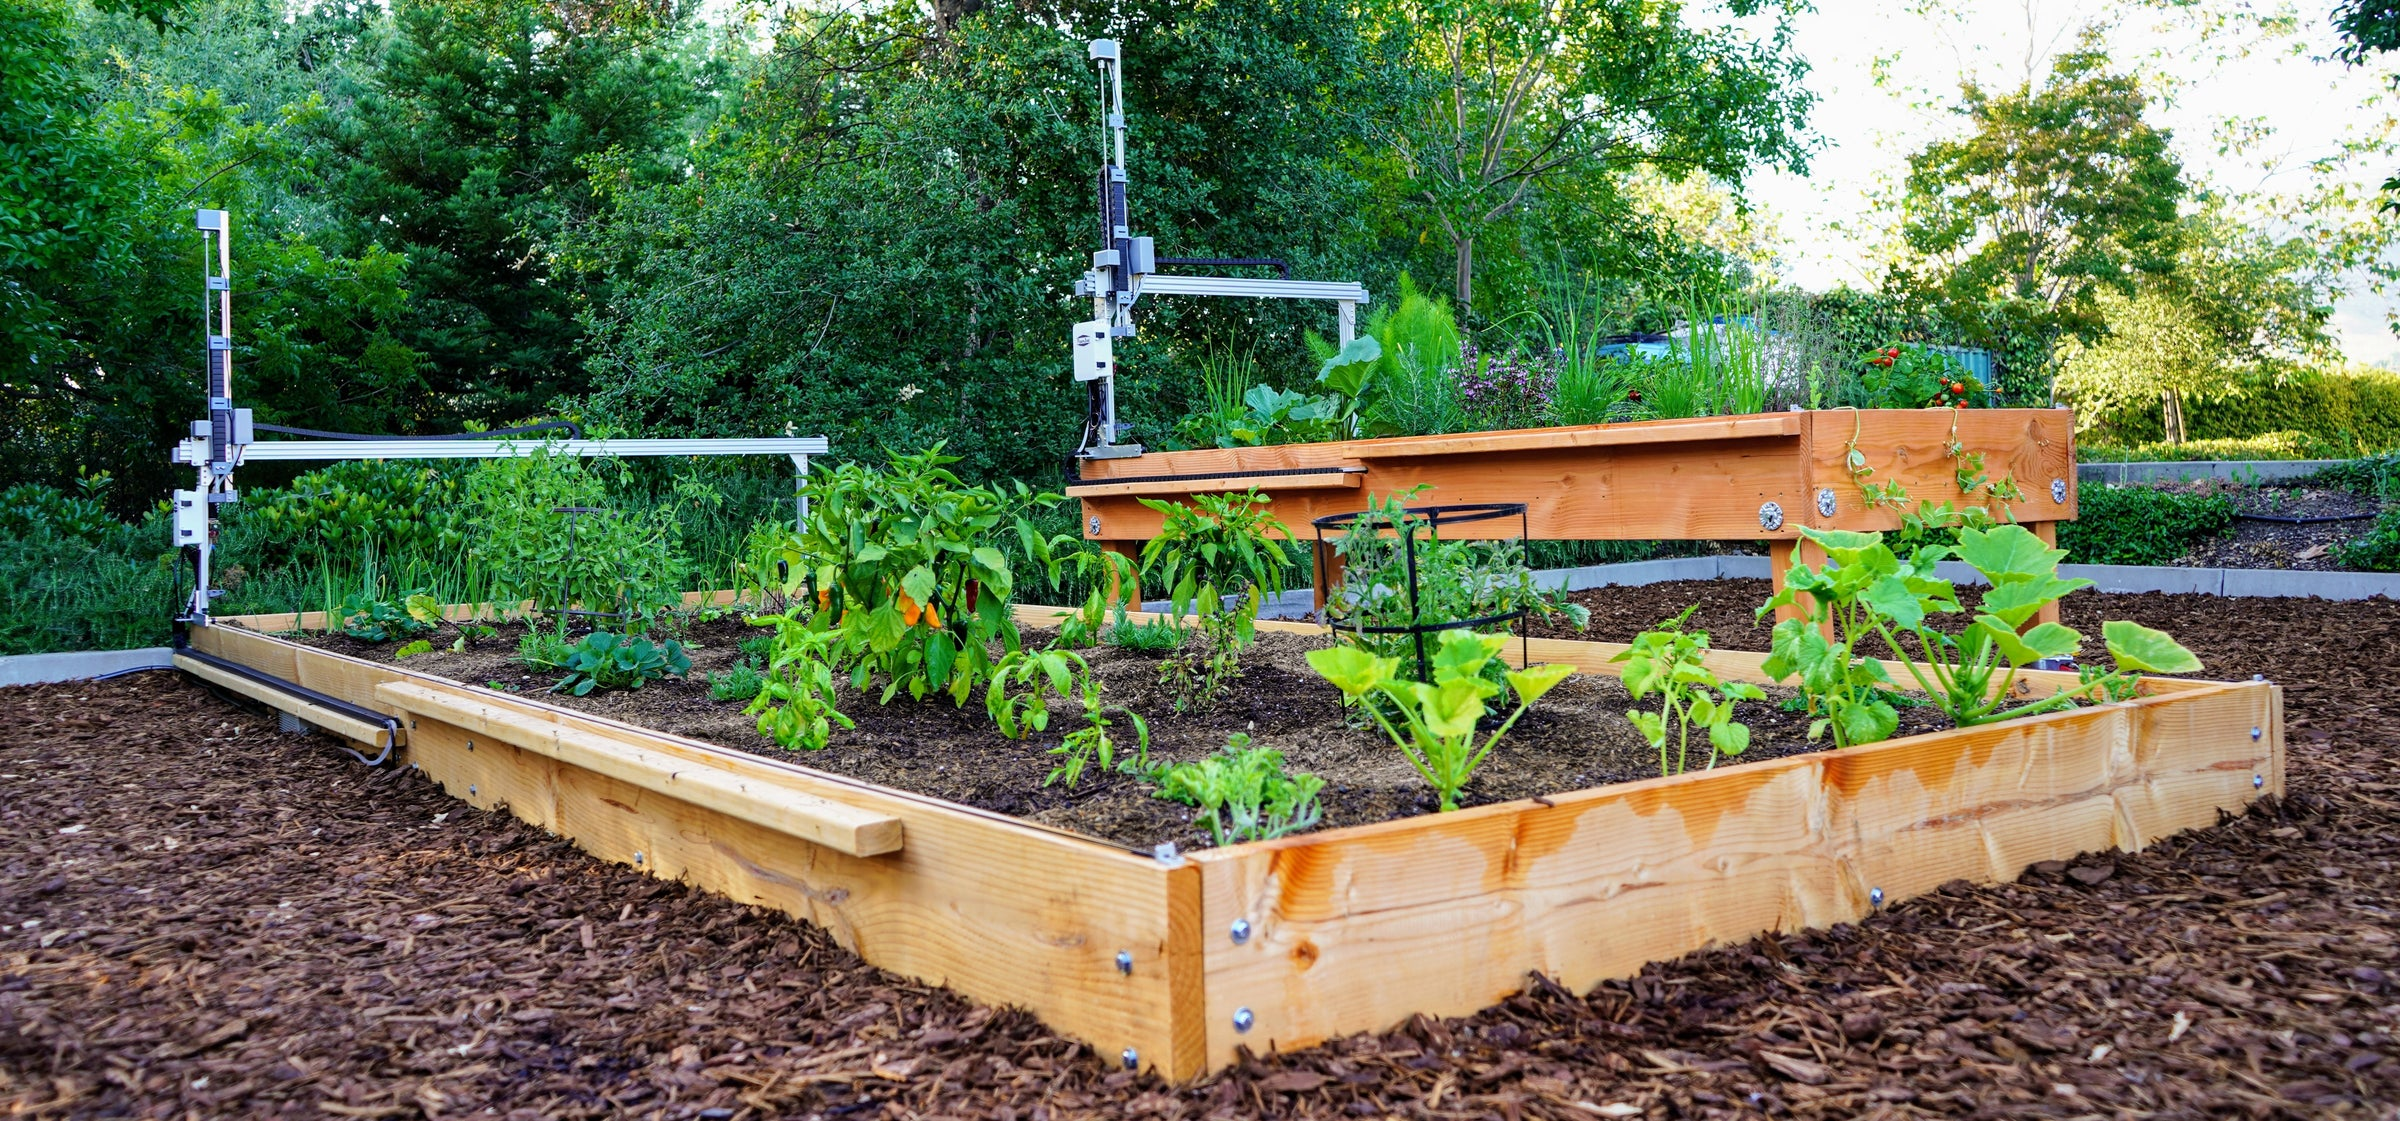
\includegraphics[width=0.5\textwidth]{bilder/farmbot.png}
	\caption[Farmbot]{Farmbot}
	\label{fig:farmbot}
\end{figure}

Der Farmbot ist ein Schienensystem, was von der Mechanik stark an einen 3D-Drucker erinnert.
Verkauft wird hierbei von dem Unternehmen nur die Hardware, sprich Schienen, Motoren, Adapter, Verkabelung und ein Raspberry Pi für die Software.\\
Die Software ist open-source, also frei im Internet für alle zugänglich, was mehrere Vorteile mit sich bringt:\\
Die Software wird von jedem User gedownloaded und eventuell umgeschrieben. Das bedeutet die Software wird kontinuierlich Probe gelesen.
Außerdem können User die Software verändern und anpassen, etwaige Fehler beheben oder Performance-Verbesserungen vornehmen.
		\section{Roboterfahrzeuge}
		Ein weiteres weit verbreitetes Konzept sind Roboterfahrzeuge mit Reifen- oder
Rollenantrieb. Diese werden hauptsächlich bei niedrig wachsenden Sorten zur
Erkennung von Schädlingen oder beschädigten Pflanzen genutzt. Dies geschieht
durch hochauflösende Kamerasysteme und der Verarbeitung der Ergebnisse, zum
Teil mithilfe von künstlicher Intelligenz.

\begin{figure}[h]
	\centering
	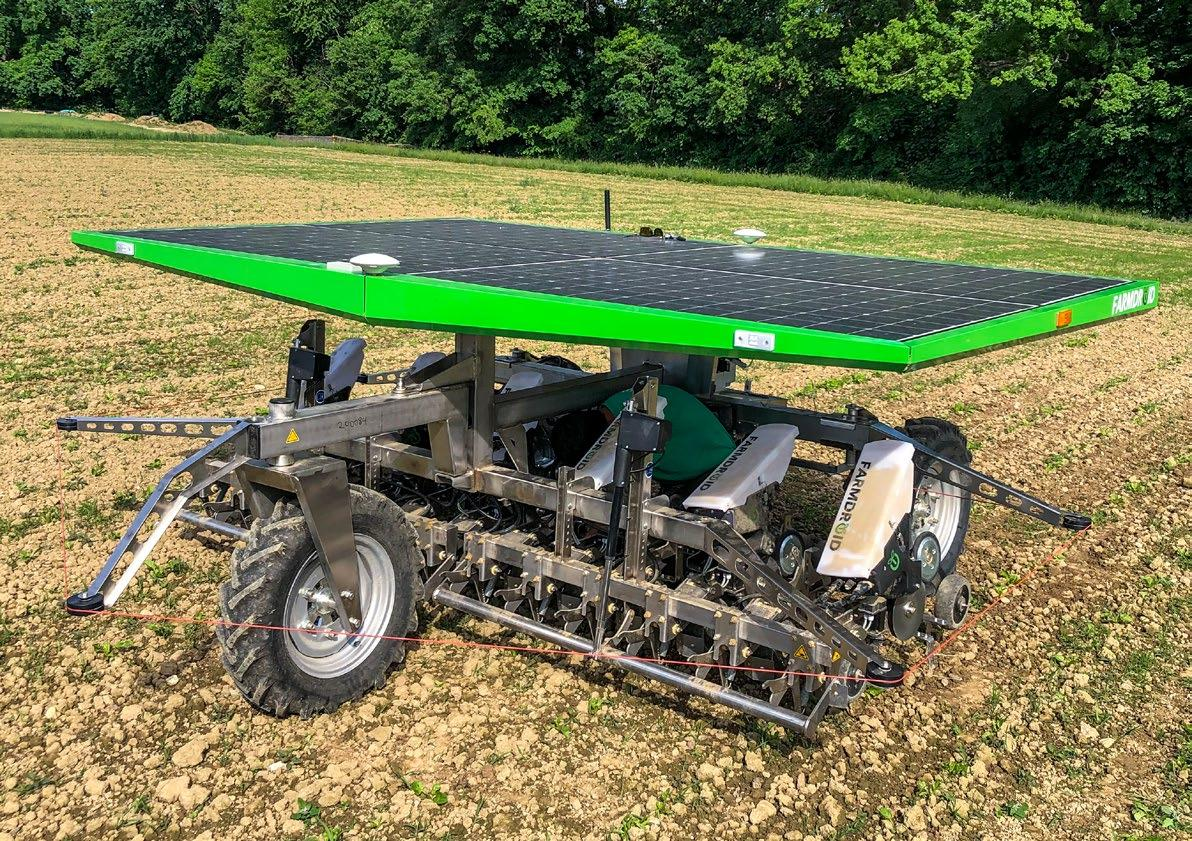
\includegraphics[width=0.7\textwidth]{bilder/farmdroid_fd20.png}
	\caption[Farmdroid FD20]{Farmdroid FD20 \cite{Wurst}}
	\label{fig:farmdroid_fd20}
\end{figure}

Der Farmdroid FD20(Abbildung \ref{fig:farmdroid_fd20}) arbeitet hierbei komplett autonom und klimaneutral durch
Solarpanels. Diese Solarpanels können bei guter Sonneneinstrahlung mehr als
genug Energie für den Roboter liefern. Durch zwei zusätzliche Lithium-Ionen
Akkus ist es möglich, dass der Farmdroid auch nach Sonnenuntergang autark
weiterarbeitet, was einen Dauerbetrieb ermöglicht und damit extrem effizient
ist.\cite{jungwirth2022arbeitszeitbedarf}\\ Die Aufgabe des modernsten
Agrarroboters der Welt\cite{donaukurier2022} ist die Saat und die
Unkrautvernichtung. Laut Hersteller hat sich der Farmdroid bereits nach bis zu
1,5 Jahren amortisiert und arbeitet ab diesem Zeitpunkt aufgrund der
Solarpanels mit extrem niedrigen Unterhaltskosten. Zudem ist der Roboter
aufgrund der zwei GNSS Empfänger und eines RTK Korrektursignals, welches in der
Basisstation erzeugt wird, sehr genau.\cite{jungwirth2022arbeitszeitbedarf}\cite{spykman2023wirtschaftlichkeitsbewertung}

	%%%%%%%%%%% BENÖTIGTE SENSOREN %%%%%%%%%%
	\chapter{Sensorik}
	
		\section{Temperatursensor}
		Wichtig für das Wachstum von Pflanzen ist natürlich die Temperatur. Je nach Herkunft benötigen Pflanzen unterschiedliche Temperaturen.\\
Um die das Absterben von Pflanzen durch falsche Temperaturen zu verhindern, benötigen Roboter zur Überprüfung Temperatursensoren.\\
Es gibt verschiedene Arten von Temperatursensoren:

\begin{description}
	\item {Temperatursensoren:}
	\begin{itemize}
		\item {\textit{IR}}
		
		\item {\textit{Thermistoren}}\\
		Thermistoren sind Bauteile, welche ihren Widerstand bei steigender Temperatur verringern. Sie bestehen aus Keramik oder Polymeren und die Temperatur wird hierbei sehr genau und schnell ausgegeben.
		\item {\textit{Widerstandsdetektoren}}\\
		Widerstandsdetektoren (RTDs) funktionieren wie Thermistoren, bestehen aber aus Metall, wie Kupfer, Nickel oder Platin. Sie sind genauer, aber auch teurer als Thermistoren. Da Pflanzen durchaus mit Temperaturschwankungen klar kommen, und nicht eine, auf 1/10°C genauere Temperatur benötigen, reichen für die Landwirtschaft Thermistoren aus.
	\end{itemize}
\end{description}


		\section{Bodenfeuchtigkeitssensor}
				Pflanzen brauchen Wasser. Je nach Sorte mehr oder weniger, nicht zu viel und nicht zu wenig. Um zu wissen, ob bewässert werden soll, benötigt der Roboter Bodenfeuchtigkeitssensoren.
		
		\begin{description}
			\item {Temperatursensoren:}
			\begin{itemize}
				\item {\textit{kapazitive Sensoren}}
				ÄNDERUNG DER DIELEKTRIZITÄTSKONSTANTE
				
				\cite{induuxwiki2022}
				\item {\textit{Leitfähigkeitssensoren}}
				Wie die meisten bereits wissen, leitet Wasser Strom. Natürlich lässt sich somit über die Leitfähigkeit der Gehalt an Wasser im Boden feststellen.\\
				Das heißt, man leitet sich wie bei Thermistoren und RTDs die Größe über den Widerstand her. Das ist auch der Grund, weshalb es viele Sensoren gibt, die Feuchtigkeit und Temperatur gleichzeitig ermitteln können.
			\end{itemize}
		\end{description}
		
		\section{Nahinfrarotspektroskopie}
		Nahinfrarotspektroskopie(NIR) verwendet Wellenlängen zwischen 780 und 2500nm,
was sich zwischen dem mittleren Infrarotbereich und dem sichtbaren
Spektralbereich befindet. Die Besonderheit bei NIR ist, dass dort die
Oberton-und Kombinationsschwingungen von Molekülen betrachtet werden.
\cite{shenk2001application} Durch die Reaktion der Moleküle auf NIR-Strahlung,
kann man viele Rückschlüsse auf die chemische Zusammensetzung von Materialien
ziehen. Bei einer Wellenlänge von 880nm kann man zum Beispiel im dritten
Oberton eine Reaktion von Fett in der Milch erkennen. \cite{cen2007theory}
Diese Technologie wird in der Landwirtschaft zum Beispiel zum Überwachen von
Futtermischverhältnissen verwendet, da man mithilfe von NIR, wie bereits
erwähnt, den Anteil an Fett, sowie den Anteil an Proteinen bestimmen kann, ohne
das Futter zu beschädigen. Ein weiteres Anwendungsgebiet ist die Getreideernte,
wobei hier der NIR-Sensor meist am Korntankrohr des Mähdreschers verbaut ist.
(Abb. 4.1) 

\begin{figure}[ht]
	\centering
	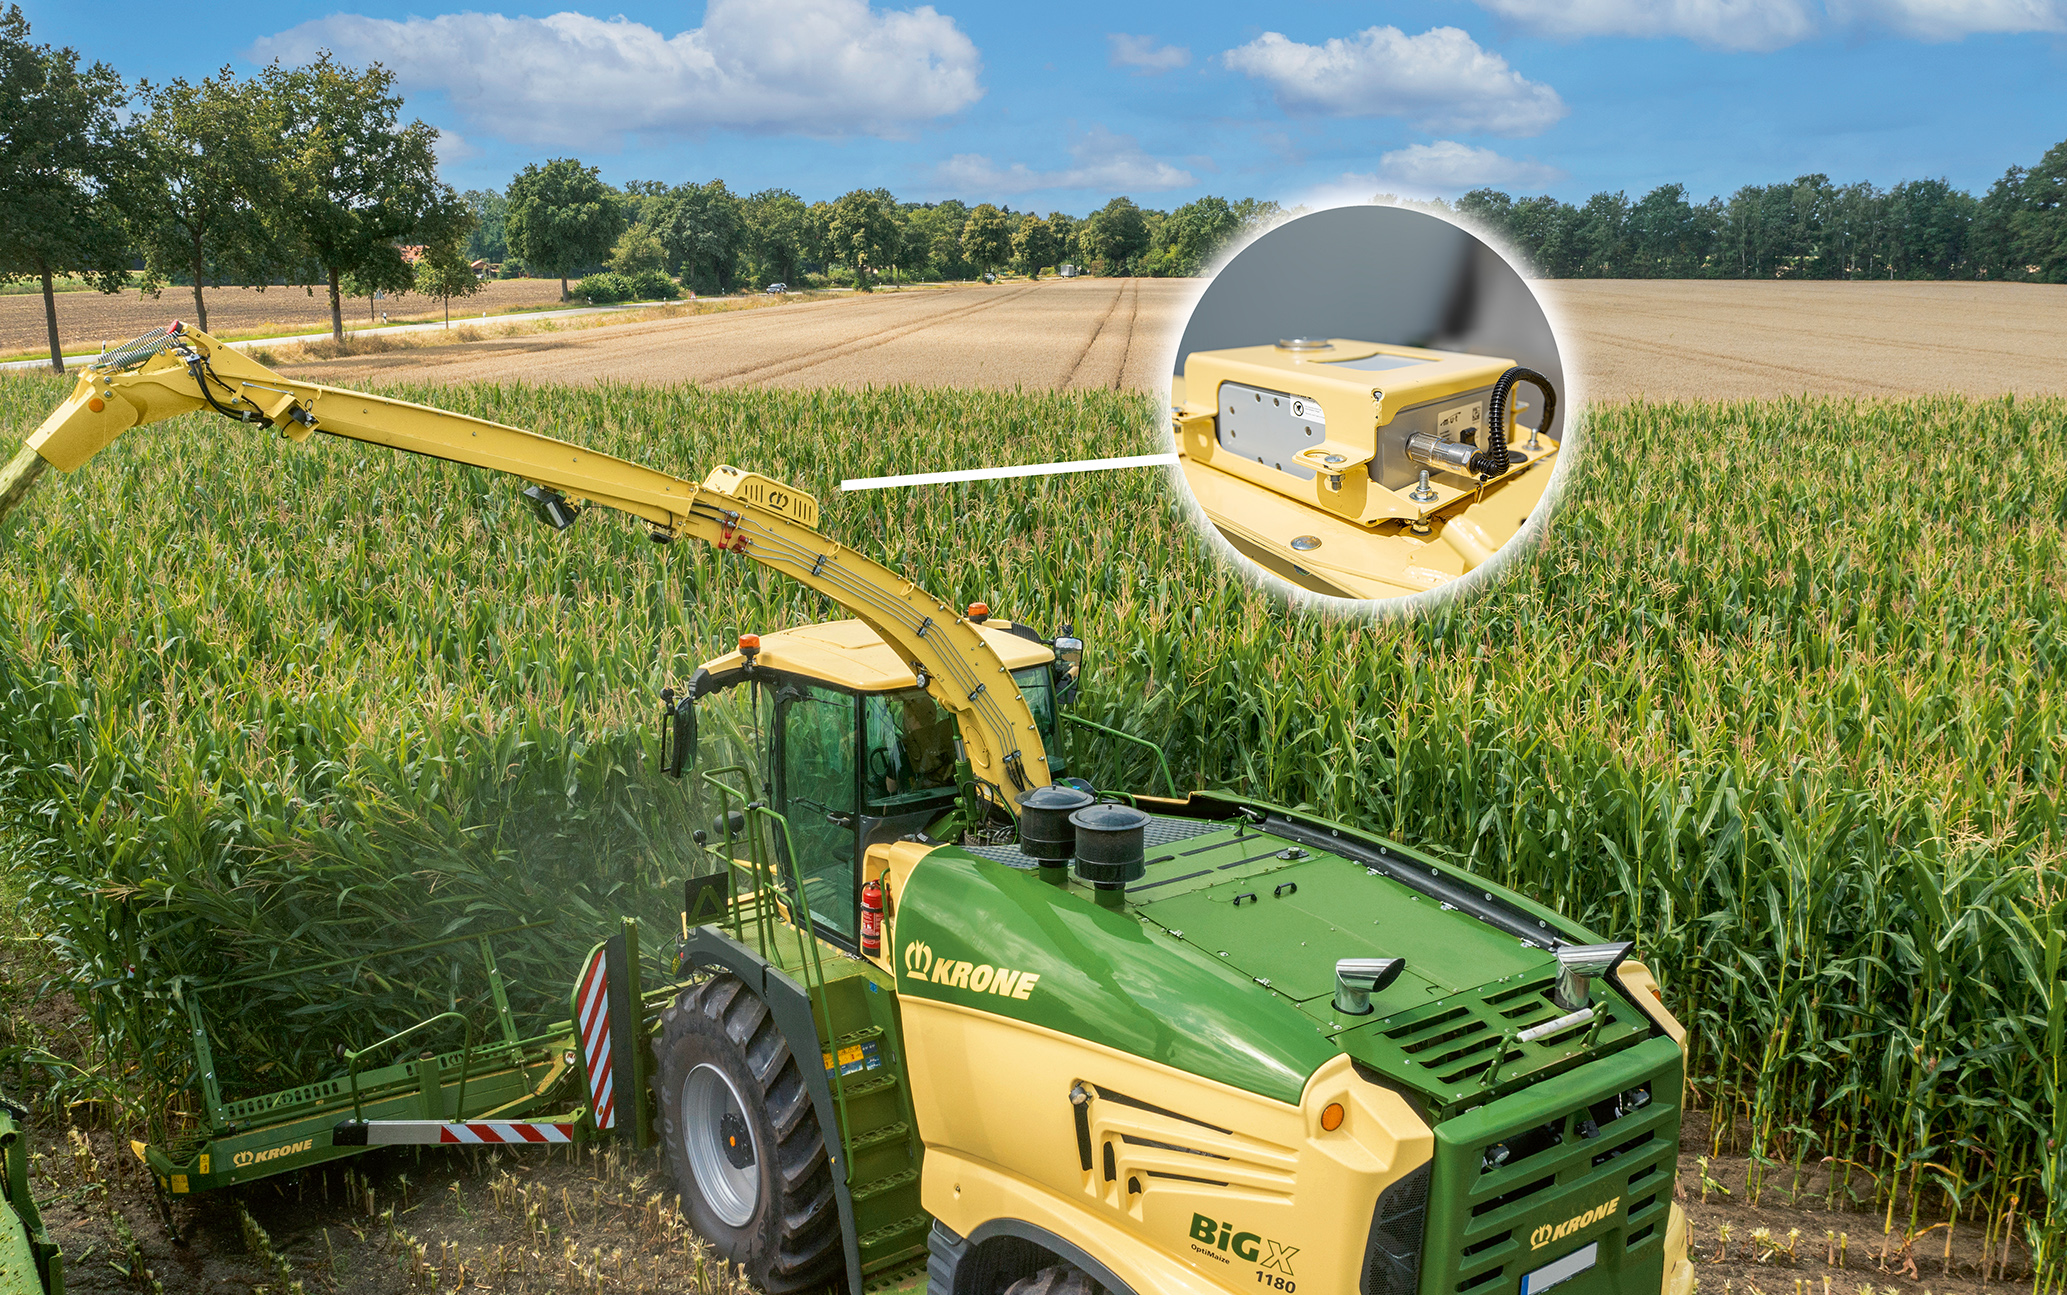
\includegraphics[width=0.5\textwidth]{bilder/Krone NIR Control dual.jpg}
	\caption[Mähhdrescher mit NIR-Sensor]{NIR-Sensor am Mähdrescher}
	\label{fig:Mähhdrescher NIR-Sensor}
\end{figure}

Er dient in diesem Fall der Überwachung der Feuchtigkeit des Saatguts,
um dieses vor Schimmel zu schützen.
	
	%%%%%%%%%%% ANWENDUNGEN %%%%%%%%%%%%%%%%%
	\chapter{Anwendungen in der Landwirtschaft}
		\section{Saat und Ernte}
		Den meisten Teil des Tages verbringt der Bauer immer noch auf dem Feld. Die einfachste Art hierfür wäre eine Automatisierung der Fahrzeuge. Das heißt ein mobiler Roboter mit Ketten- oder Reifenantrieb, würde durch fest übergebene GPS-Daten Bahnen im Feld abfahren und ernten, bzw. sähen. \\
Ein wichtiger für das Sähen benötigter Sensor ist ein Ultraschallsensor, zum Messen der Bodenentfernung. Damit können die Samen auf die exakte Tiefe in den Boden eingebracht werden.\\
Beim Ernten kommt es vorallem auf die Sorte an. Hierbei kommt es weniger auf die Sensorik, als auf die Aktorik an. Das liegt daran, dass alle Pflanzen bei der Ernte ziemlich gleich groß sind, innerhalb ihrer Sorte, welche im Vornherein bekannt ist. Dabei werden die Pflanzen komplett "abgeschnitten". Man könnte jedoch bereits beim Erntevorgang durch eine Bildverarbeitung beschädigte, kaputte Ernte aussortieren. Hierfür wäre vorallem ein sehr gutes Kamerasystem nötig, wobei man jedoch Kosten-Nutzen hierbei beachten sollte, da ein komplexes Kamerasystem schnell sehr teuer werden kann.
		\section{Tierpflege}
		Der Großteil, neben der Feldarbeit, dreht sich bei der Landwirtschaft um den
Viehbetrieb. Hier gibt es bereits einige Automatisierungen, wie zum Beispiel
Melkstraßen, wo Kühe mithilfe von Melkrobotern nacheinander vollautomatisch
gemolken werden. Was zudem sehr leicht zu automatisieren ist, ist die Ernährung
jeglicher Tierarten.\\ Man benötigt lediglich ein System, das Futter von großen
Lagerbehältern zu den Ställen/Gehegen bringt. Das kann je nach Bauernhof
unterschiedlich aussehen. Die einfachste Umsetzung wäre hierbei meiner Hinsicht
nach ein höher gelegenes Schienensystem. Damit gibt es keine Behinderung der
sonstigen Arbeit, und man kann das komplette System mittels eines
Mikrokontrollers, wie zum Beispiel eines Raspberrys, steuern. Die
herkömmlichsten Roboter gleichen jedoch herkömmlichen Futtermischwägen, welche
vollautomatisiert durch die Ställe fahren. (Abb. 5.1)

\begin{figure}[ht]
    \centering
    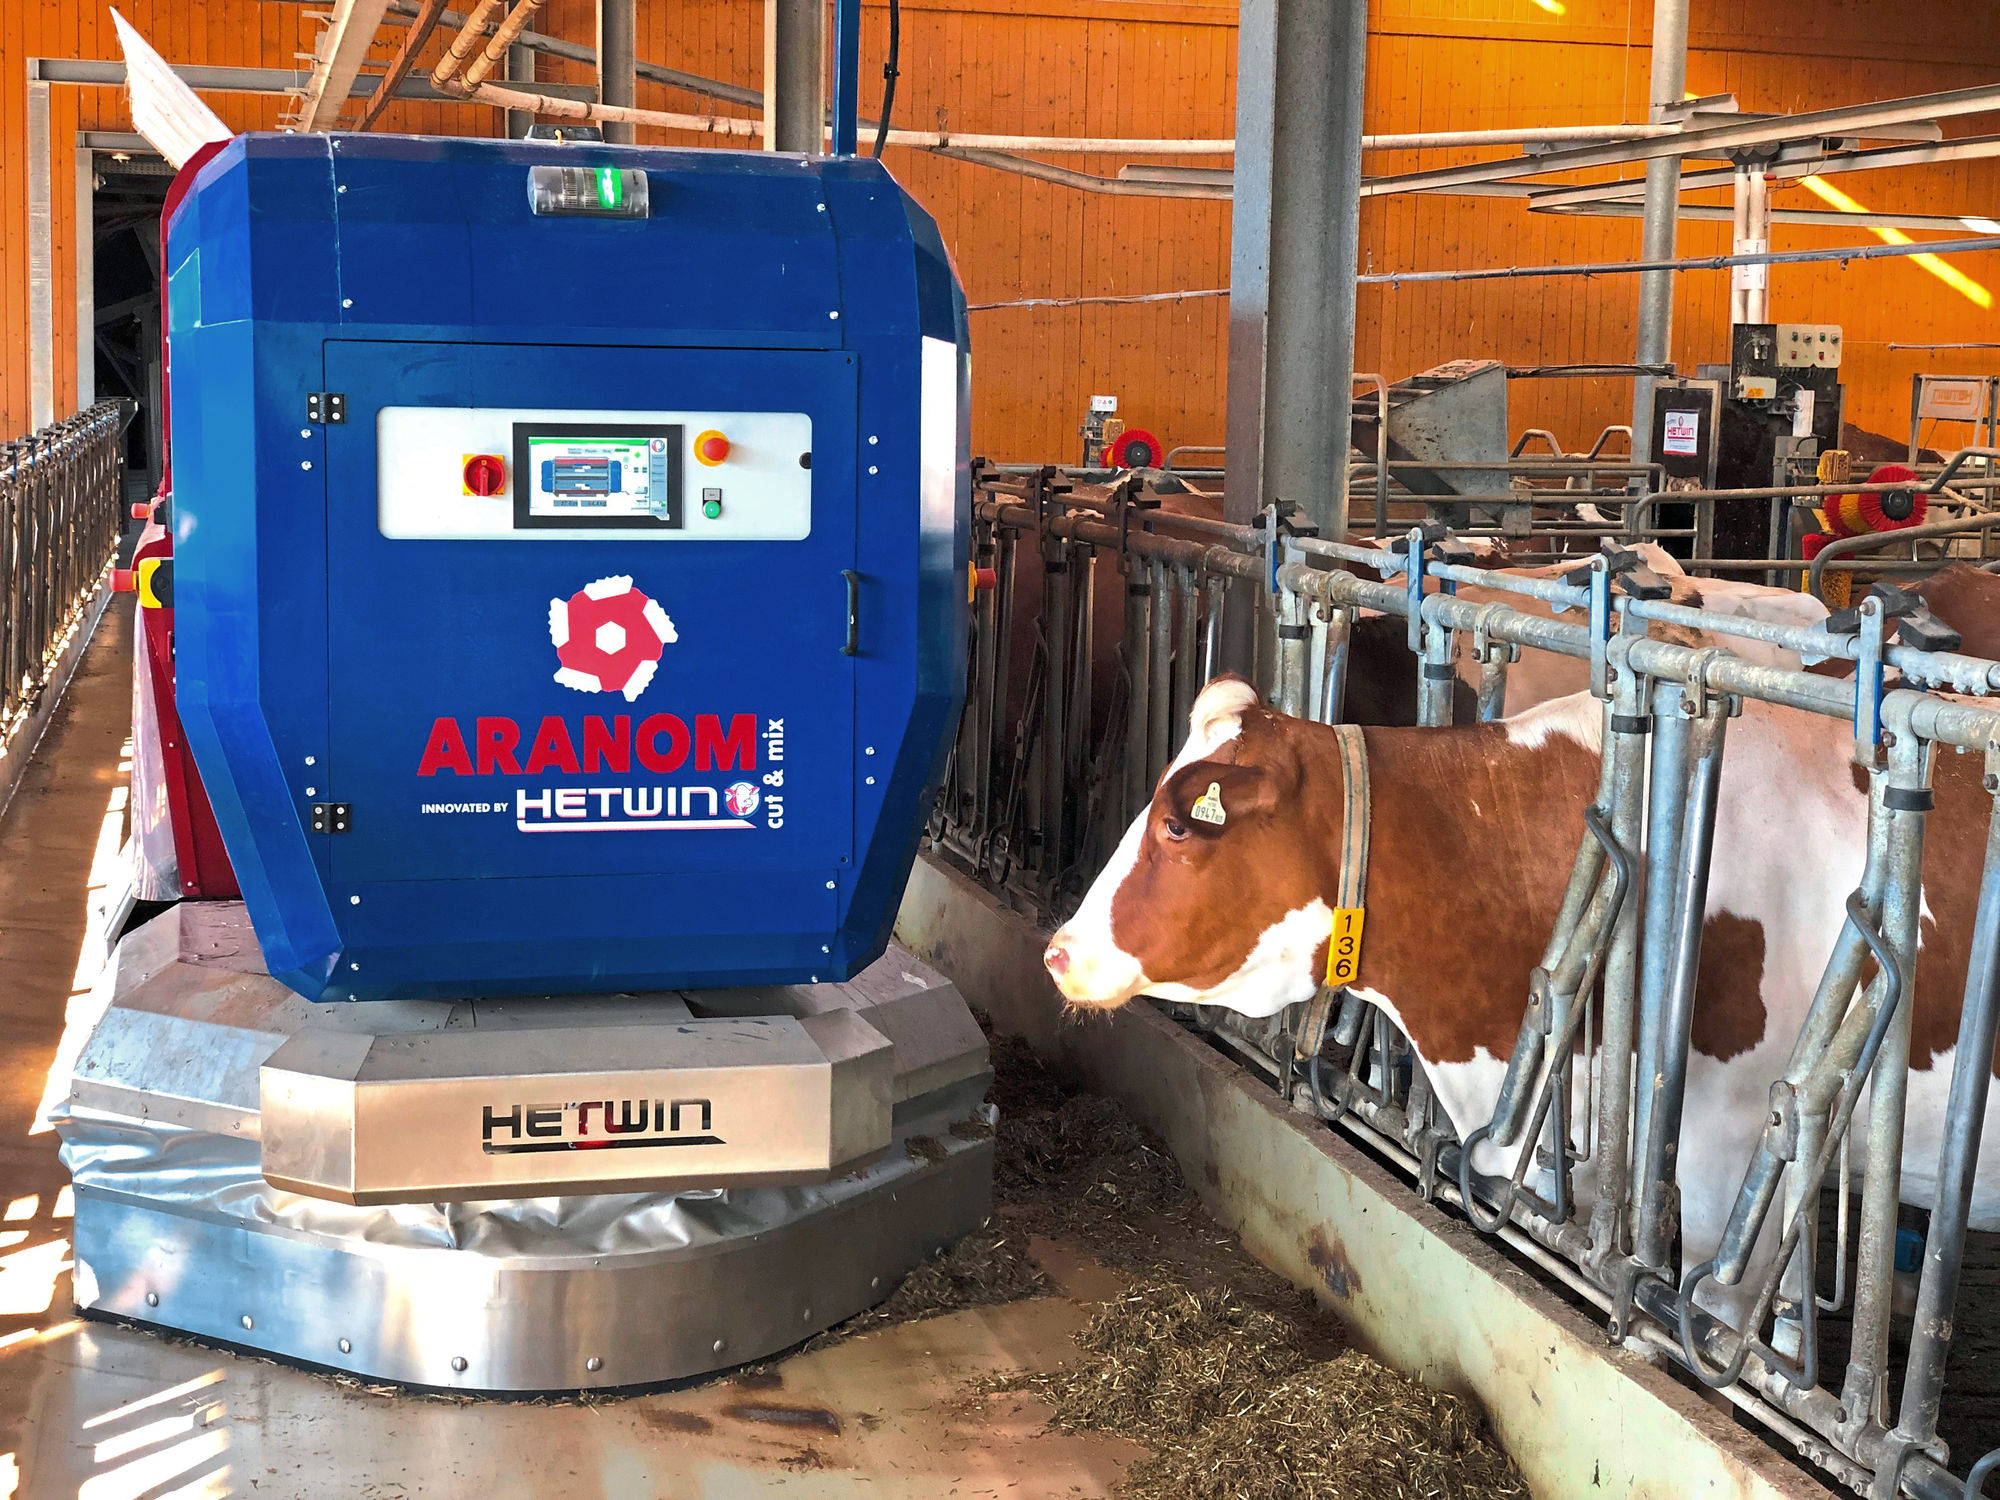
\includegraphics[width=0.5\textwidth]{bilder/futterroboter.jpg}
    \caption[Futterroboter in Kuhstall]{Futterroboter in Kuhstall}
    \label{fig:sprühdrfutterroboter}
\end{figure}
		\section{Bodenpflege}
		Zur Bodenpflege gehören die Analyse von Mineralstoffen, Bodendichte und
Bodenbeschaffenheit. Wie der Name schon sagt, wird bei dieser Arbeit ein
Mineralwertsensor benötigt.\\	
		\section{Bewässerung}
		Eine weitere Anwendung, welche in der Landwirtschaft in Kombination mit
Sensorik viel Einsatz findet ist Bewässerung. Vorallem durch das immer weniger
werdende Grundwasser, sind Pflanzen auf eine externe Bewässerung angewiesen.
\cite{liu2018self} Bewässerung kann auf unterschiedliche Arten realisiert
werden. Man unterscheidet zwischen Flächenbewässerung und punktueller
Bewässerung. Flächenbewässerung wird meist mit Sprenklern realisiert die mittig
aufgestellt werden und so die Pflanzten von oben mit Wasser versorgen. Vorallem
in sehr heißen Gebieten ist das recht ineffizient, da ein Großteil des Wassers
auf der Pflanze verdunstet, bevor es aufgenommen werden kann. Ein sehr viel
besseres System für die Freiflächenanwendung sind Schläuche, welche in
Bodennähe verlegt werden. Mit vereinzelten Löchern wird durch den Schlauch
Wasser abgegeben, welches direkt vom Boden aufgenommen werden kann und unter
dem Pflanzen, geschützt vor der Sonne, nicht verdunstet. Der Nachteil an
Schläuchen im Freien ist die Anfälligkeit gegenüber Zerstörung durch Tiere,
besonders Marder neigen dazu, Schläuche aufzubeißen, womit eine Verluststelle
im System besteht, die nur schwer bemerkt und lokalisiert werden kann. Einen
weiteren Aspekt, den es zu beachten gilt, wenn Felder in freier Umgebung
bewässert werden sollen, ist die dauerhafte Überwachung der Bodenfeuchtigkeit.
Wenn es regnet, neigt ein bewässertes System schnell zur Überwässerung. Durch
Bodenfeuchtigkeitssensoren (Kapitel 4.2) kann mithilfe eines Mikrokontrollers
ein Feuchtigkeitsthreshold eingestellt werden, welcher sicherstellt, dass die
Pflanzen genau die richtige Menge an Wasser bekommen. Außerdem gibt es Ansätze,
zur passiven Versorgung mit Wasser, wobei man versucht, das Optimum aus
Niederschlag und Grundwasser zu nutzen. Ein Beispiel hierfür beschäftigt sich
mit der Idee ein T-Stück im Boden einzusetzen. Der obere Teil des T-Stücks soll
das schnelle versickern des Niederschlags verhindern, womit die Pflanzen mehr
Zeit haben diesen mithilfe der Wurzeln zu verwenden. Der untere Teil des Teils
reicht bis zum Grundwasser. Wie bereits vorher erwähnt, ist der
Grundwasserspiegel inzwischen zu niedrig, um von den Pflanzen erreicht zu
werden. Mithilfe von kleinen Röhren wird die Kapillarkraft verwendet, um
Grundwasser von unten, nach oben zu den Pflanzen zu transportieren, wobei das
vollkommen autonom und ohne jegliche Ansteuerung funktioniert. \cite{liu2018self}	
		\section{Schädlingsbekämpfung}
		Meist werden Schädlinge, wie Parasiten und Unkraut mithilfe von Pestiziden
bekämpft. Diese werden meist unter Zuhilfenahme von Traktoren auf dem Feld
ausgebracht. Ein neuerer Ansatz ist die Verteilung mit Drohnen, die wie bereits
erwähnt die Flüssigkeit aus der Höhe weitflächig auf den Feldern verteilen
könnten. Jedoch ist aufgrund der Gefahr von Verwehung die maximale Flughöhe auf
2m über den Pflanzen, sowie die Geschwindigkeit auf 13km/h
beschränkt.\cite{bvl} Somit erübrigt sich dieser Vorteil, was jedoch bleibt ist
die fehlende Bodenzerstörung durch Reifen, welche bei einer traktorbasierten
Ausbringung der Fall wäre. Auch in der Atemluft lagern sich Pestizide ab, was
bereits 2019 in einer Studie nachfgewiesen wurde, in welcher Baumrinde
untersucht wurde, wobei man in 47 Proben 104 verschiedene Pestizide finden
konnte.\cite{clausing2020baumrinden}

	%%%%%%%%%%%% HERAUSFORDERUNGEN %%%%%%%%%%
	\chapter{Künstliche Intelligenz}
	\input{kapitel/künstliche Intelligenz.tex}
	%%%%%%%%%%% FAZIT %%%%%%%%%%%%%%%%%%%%%%%
	\chapter{Fazit}
	Zusammenfassend kann davon gesprochen werden, dass auch die Landwirtschaft von dem
Umschwung in die Automatisierung von Prozessen betroffen ist. Vorallem in
dieser Branche gibt es viele gute Möglichkeiten, Systeme mithilfe von Sensoren
zu überwachen und zu beeinflussen. Auch mit dem Hintergrund des
Bevölkerungswachstums und der damit einhergehenden Steigerung des Mangel an
Lebensmitteln ist es besonders wichtig, jede Chance zu nutzen, die
Landwirtschaft so effizient wie möglich zu gestalten. Auch den Aspekt, der
Zerstörung des fruchtbaren Boden muss beachtet werden, beim Gedanken an die
Ernährung der immer größer werdenden Menschheit.\cite{rainer2003diskurs}
Systeme wie der Farmbot helfen, jeden freien Platz sinnvoll zu nutzen und
animieren die Menschen, auch Zuhause Pflanzen selbst zu züchten. Jedoch muss
dies in einem für die Umwelt möglichst erträglichen Rahmen geschehen. Hierfür
sind die Roboter eine große Hilfe, die zum Großteil, im Gegensatz zu den alten
dieselbetriebenen Landmaschinen, durch elektrische Antriebe bewegt werden.
Durch Solarmodule können diese immer weiter nahezu autark und emissionsfrei
arbeiten, was eine hohe Entlastung für die Umwelt darstellt. Dass die
konservative Landwirtschaft immer mehr Technik einsetzt, zeigt sich bereits an
einigen Umfragen. 
Auch gesundheitlich kann die Digitalisierung der
Landwirtschaft viele Vorteile bieten. Durch den Verzicht auf Pestizide, bzw.
die Ausbringung durch Drohnen aus der Ferne, wird die Gesundheit der Bauern
geschont, da sie die giftigen Pestizide nicht einatmen.
\cite{jungwirth2022arbeitszeitbedarf}
	%%%%%%%%%%% INHALTSVERZEICHNIS %%%%%%%%%%
	\printbibliography
	%%%%%%%%%%% ABBILDUNGSVERZEICHNIS %%%%%%%
	\listoffigures
\end{document}
%% im fließtext bei Zitat auf Autor beziehen %%